\section{Statement} \label{sec: stat}

The statement of the curret project can be found in \cite{enunciado}. The aim is to define the structural behavior of a determined asrospace structure, that is modelled by three aluminum thin panels ($L_1=1.25$ m,$L_2=1$ m and $t=5\cdot 10^{-3}$ m, see \autoref{fig: enunciado}) with a separation $t = 5\cdot 10^{-2}$ between them, forming two air layers. The properties of the panels are defined on \autoref{tab: panel} whereas the air layer's ones  can be seen on \autoref{tab: air}.


\begin{figure}[htpb]
 \centering
    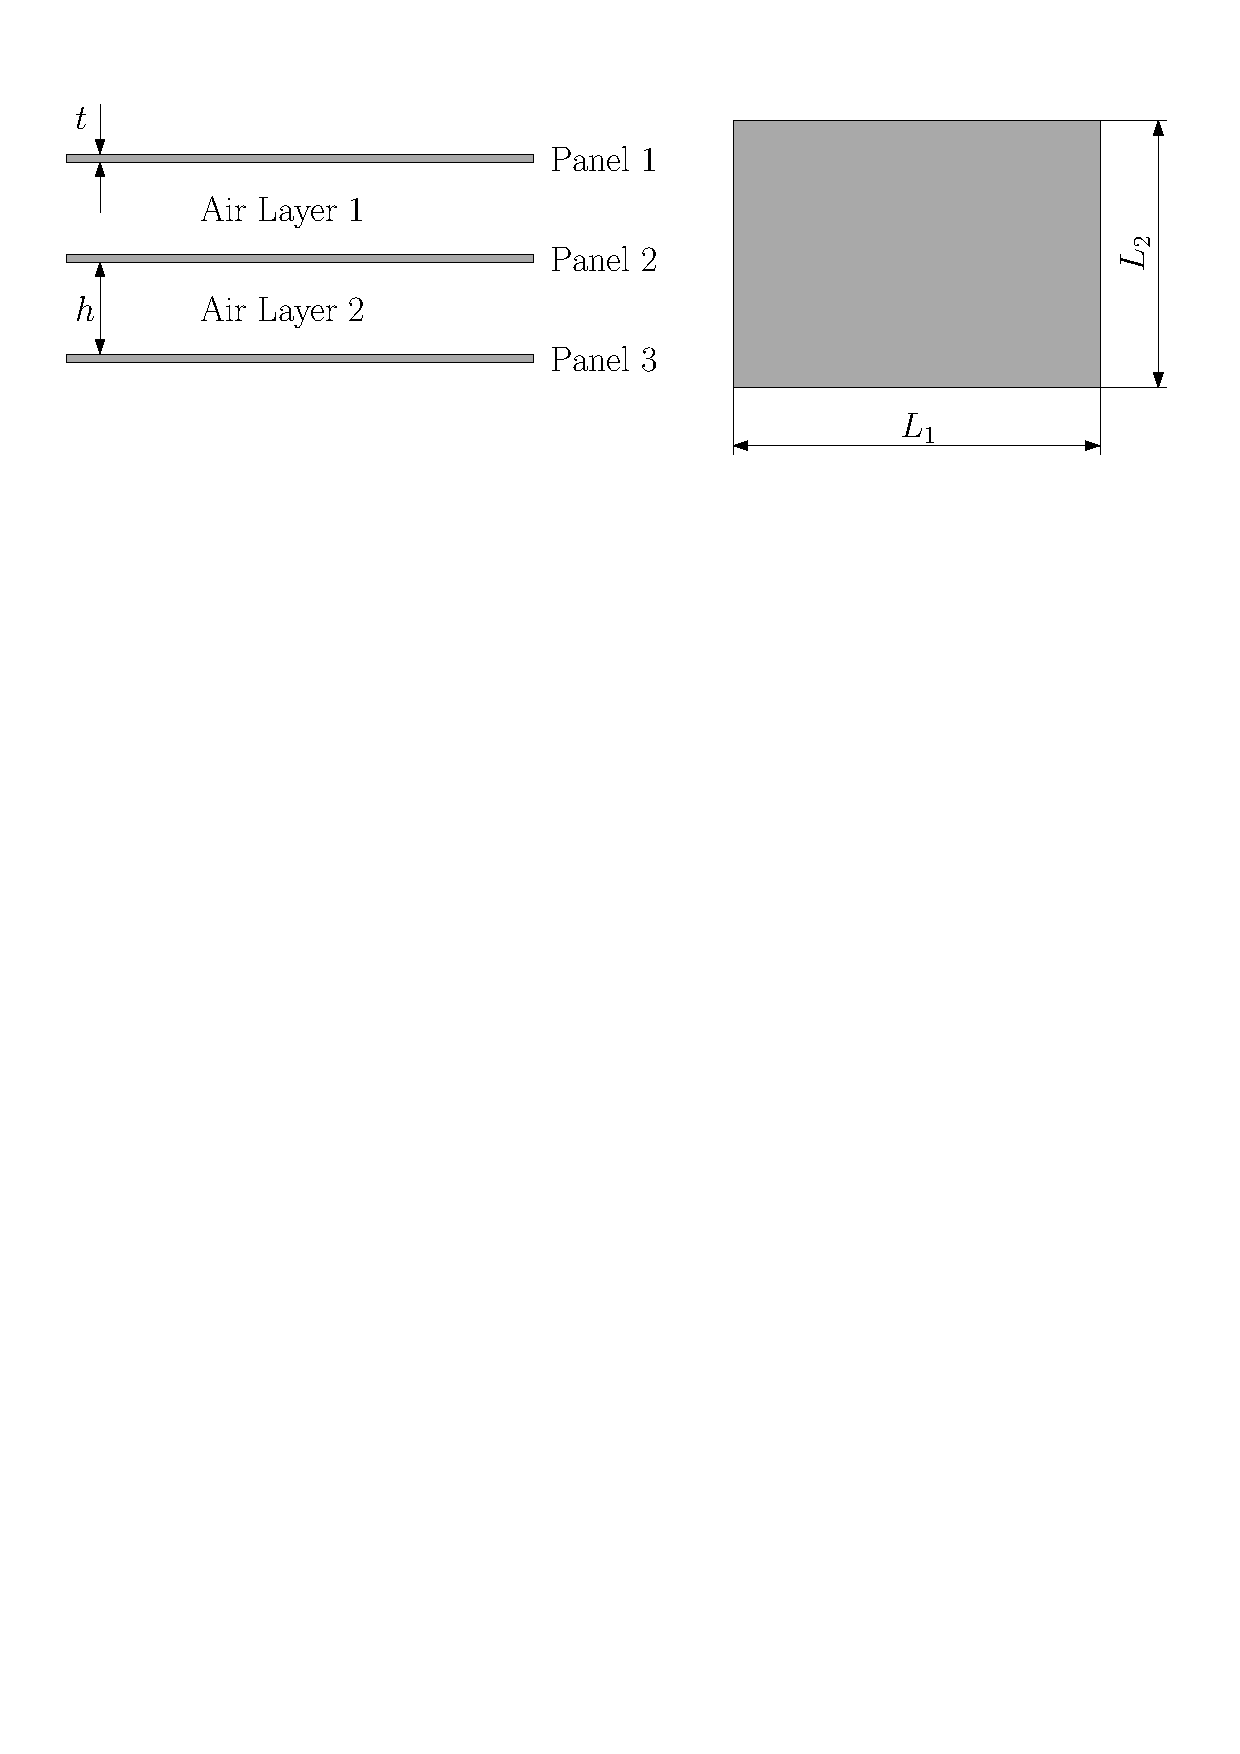
\includegraphics[scale=0.75]{Figures/enunciado.pdf}
  \caption{System of analysis.}
  \label{fig: enunciado}
\end{figure}

\begin{table}[h]
    \caption{Panel properties.}
    \label{tab: panel}
    \centering
    \begin{tabular}{ccc}
    \toprule 
        $\boldsymbol{\rho} 		[\frac{\text{kg}}{\text{m}^3}]$  & $\boldsymbol{E} [\text{Pa}]$ &$\boldsymbol{\nu}[-]$ \\
        2700 & $70\cdot 10^{9}$ & 0.33 \\
       
        \bottomrule
    \end{tabular}
\end{table}

\begin{table}[h]
    \caption{Air properties.}
    \label{tab: air}
    \centering
    \begin{tabular}{cc}
    \toprule 
        $\boldsymbol{\rho} 		[\frac{\text{kg}}{\text{m}^3}]$  & $\boldsymbol{c_0} [\frac{\text{m}}{\text{s}}]$  \\
        1.23 & 343 \\
        \bottomrule
    \end{tabular}
\end{table}

The objective is to calculate the average velocity of the panels and the mean quadratic pressure in the air layers at a high- frequency range,  taking into consideration an external excitation on the panels whose distribution is presented in \autoref{tab: potencia}.

\begin{table}[h]
    \caption{Distribution of external power applied on each panel.}
    \label{tab: potencia}
    \centering
    \begin{tabular}{cccc}
    \toprule 
        $\boldsymbol{f} $ \textbf{Hz} &  $\boldsymbol{P_{1}}$ \textbf{[W]} &  $\boldsymbol{P_{2}}$ \textbf{[W]}&  $\boldsymbol{P_{3}}$ \textbf{[W]} \\
        $16 \leq f \leq 1000$ & 10 &  &  \\
        1250 & 20 & 8.7000 & 20\\
		1600 & 35 & 15.2000 & 35\\ 
		2000 & 50 & 21.7400 & 50\\ 
		2500 & 80 & 36.9600 & 80\\ 
		3150 & 100 & 39.1300 & 100\\ 
		4000 & 150 & 45.6500 & 150\\ 
		$5000 \leq f \leq 10000$ & 100 & 43.4700 & 100\\ 
        \bottomrule
    \end{tabular}
\end{table}

To compute the system response, the following steps must be followed:
\begin{itemize}
\item Calculate the number of modes per bandwidth as a function of frequency for the panels and for the air layers. Specify the frequency from which all the elements of the system can be represented by energetic models, assuming that the high-frequency condition is set at $N \geq 5$ modes.
\item Calculate the cross- coupled dmpling terms ($\eta_pa$ and $\eta_ap$) as a function of frequency.
\item Write down the equations of the SEA model that consist of the 3 panels (only taking into account the bending modes) and the two air layers.
\item Compute and represent the energy  as a function of frequency.
\item Calculate the average speed of the panels and the root mean square pressure of the air as a function of frequency.
\end{itemize}


